\graphicspath{{capitulos/Capitulo3-Metodologia-propuesta/recursos/}}

\section{Metodología propuesta} \label{apartado:3}
En este capítulo se describe en detalle la metodología propuesta para resolver el problema planteado en la \hyperref[apartado:2]{sección anterior}, entendiendo por metodología el conjunto de decisiones previas a la implementación tomadas con el fin de plantear una forma de resolver dicho problema.
\\

La hipótesis de partida (\hyperref[H2]{H2}) plantea como punto de comienzo del proyecto el uso de una metaheurística con el fin de optimizar todos los parámetros del sistema, pero hemos de definir dichos parámetros antes de poder definir la metaheurística.
\\

Para comenzar con el planteamiento de la metodología, podemos comenzar desde el punto de vista de la ingeniería: verlo como un sistema de caja negra que recibe una entrada y una salida.
El sistema debe poder corregir la planificación de controladores de ese día, por lo tanto es claro que la entrada será esa planificación. Recordemos que el sistema \legacy{} será empleado por el personal del aeropuerto para realizar la planificación de forma automatizada, por lo que \textbf{la entrada del sistema deberá tener un formato común con la salida del sistema \legacy{}}.
Respecto a la salida, deberá ser de un formato comprensible por el personal gerente de los puestos de control.
\\

Por último resta detallar la parte más importante: la \textit{caja negra} propiamente dicha. Pues bien, como hemos dicho antes, en primer lugar el sistema recibirá una \textbf{solución inicial}, que deberá ser tratada de acuerdo a las contingencias habidas. Por ejemplo ocurre un cambio de sectorización en mitad del turno que no estaba planificado. 
A partir del momento en el que se cierra debemos eliminar todas las apariciones de los sectores que se cierran y añadir los que se abren, pero no antes de dicho momento (mas detalles en el \autoref{sec:3:inicializacion-soluciones}). 
Llamaremos al momento en el que sucede la incidencia como \textbf{momento actual} para simplificar, aunque lo habitual es que el sistema sea ejecutado varios minutos antes de que suceda la incidencia.

Una vez tratada la solución inicial, la metaheurística ya podrá dar comienzo sobre ella, buscando diferentes 
planificaciones alternativas (soluciones) y dando como resultado la mejor. 
\\

%Con todo, el sistema tiene cuatro módulos:
%\begin{itemize}
%	\item Módulo de lectura de datos: lleva a cabo las tareas de lectura e inicialización de estructuras de datos.
%	\item Módulo de inicialización: inicializa la solución inicial de acuerdo a la(s) contingencias recibidas del módulo anterior
%	\item Módulo de búsqueda: lleva a cabo la búsqueda de una solución factible al problema.
%	\item Módulo de entrega de datos: lleva a cabo las tareas de escritura y trazabilidad de las soluciones.
%\end{itemize}

Sin entrar en detalles de implementación (para ello ver el \autoref{apartado:4}), el sistema tiene, claramente, dos 
\textit{Fases}:
\begin{itemize}
	\item \label{Fase 1} Fase 1: tratamiento de la solución
	\item \label{Fase 2} Fase 2: resolución del problema
\end{itemize}

En adelante aludiremos a la fase del sistema que comprende la inicialización de la solución de entrada según las necesidades del caso concreto de incidencia que se produzca como \faseuno{} o \textit{Fase de Inicialización}. 
Mientras que la \fasedos{} o simplemente \textit{Metaheurística}, será la fase del sistema en la que se resolverá el problema propiamente dicho de acuerdo a las pautas establecidas en forma de restricciones y puntuaciones sobre la metaheurística.
En los próximos apartados definiremos cada una de estas Fases en detalle.

\subsection{Representación de las soluciones}
Antes de entrar en detalle, es importante explicar cómo se han representado las soluciones. Recordemos que estamos representado planificaciones, es decir una relación matricial de sectores con trabajadores a lo largo del tiempo que dura un turno. De forma que dada una lista de controladores, en cada instante de tiempo tendremos un sector asignado así como el tipo de puesto (planificador o ejecutivo).
\\

\begin{figure}
	\centering
	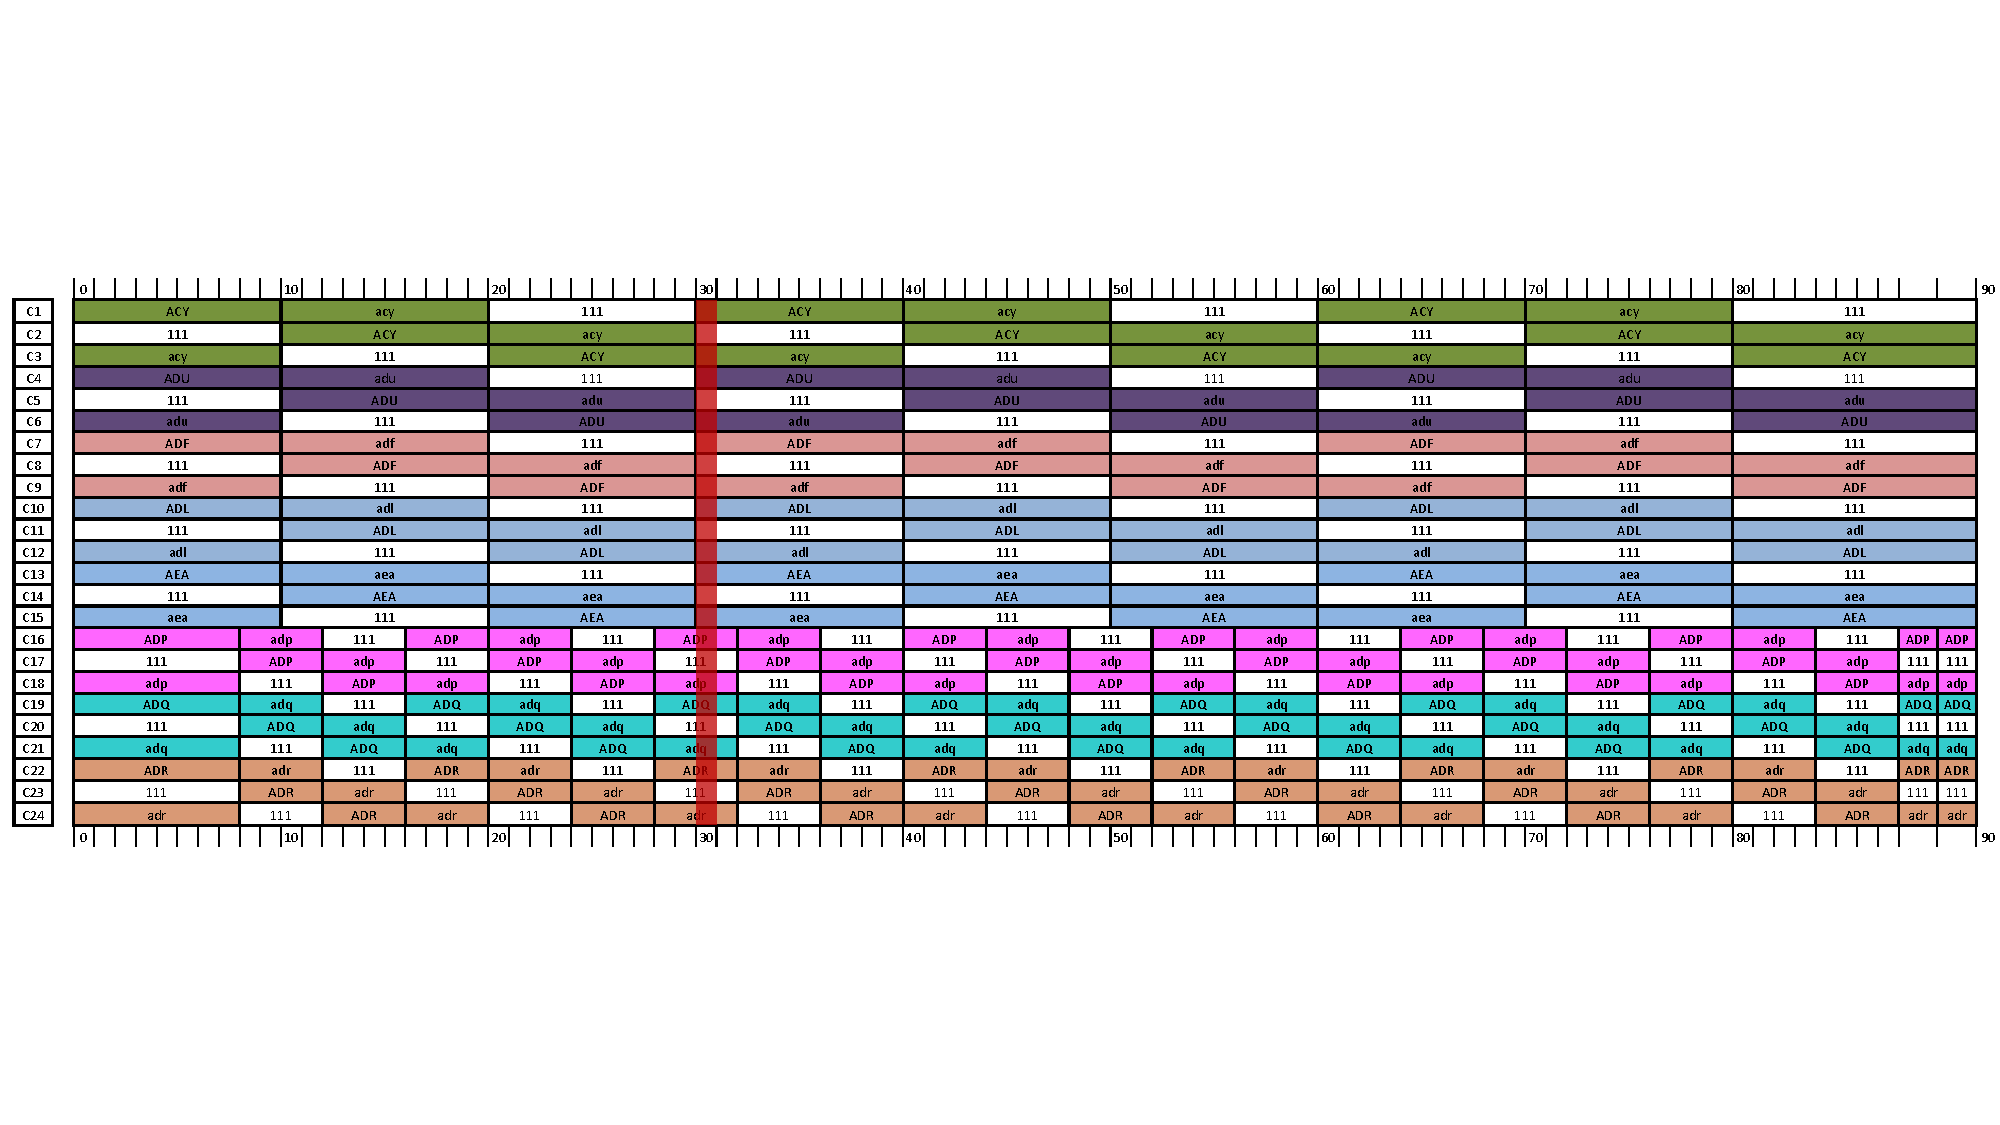
\includegraphics[width=\linewidth]{Ejemplo-distribucion-inicial}
	\caption[Ejemplo de una solución inicial]{Ejemplo de una posible solución inicial. Constituida mediante el uso 
		de plantillas. 
		Nótese que se emplean identificadores en vez del nombre completo de cada sector para abreviar}
	\label{fig:3:ejemplo-distribucion-inicial}
\end{figure}

Las filas de la matriz serán por tanto los controladores que tengamos a nuestra disposición así como los que añadamos dinámicamente para facilitarla inicialización y que serán eliminados en la \fasedos{}, mientras que las columnas de la matriz representará el tiempo (véase \autoref{fig:3:ejemplo-distribucion-inicial}) desde el inicio del turno hasta el final del turno. Por lo que el tamaño de cada una dependerá de la instancia concreta del problema que estemos 
resolviendo.
\\

El tiempo es una variable continua, que nos permitiría conocer el sector que controla un trabajador para un momento exacto del tiempo como por ejemplo las 8:29:17 (horas, minutos, segundos), una precisión del todo innecesaria en éste problema, pero también difícil de representarlo en éste tipo de problemas de \textit{timetabling}. Para poder 
representar el tiempo, debemos convertir la variable continua en discreta mediante el proceso denominado 
discretización: renunciamos a la precisión del tiempo fragmentándolo en intervalos de tiempo uniformes que llamaremos \textit{slots}, por ejemplo de 5 minutos cada uno.
\\

Esta discretización nos hace perder precisión, por lo que el tamaño del slot deberá ser el adecuado para no perder capacidad de representación en nuestras soluciones y por ende limitar espacio de búsqueda en exceso, lo cual podría desembocar en que una buena solución no pueda ser representada y por lo tanto no será contemplada por el sistema de búsqueda así que nunca se dará como solución.
En nuestro caso, hemos elegido un tamaño de slot de 5 minutos debido a que se trata del máximo común divisor de todas las restricciones numéricas del dominio del problema (ver %TODO REFERENCIAS!!!)

\begin{figure}[htbp]
	\begin{subfigure}{\linewidth}
		\centering
		
\includegraphics[width=\linewidth]{tiempo-continuo}
		\caption{Tiempo continuo}
		\label{fig:timepo-continuo}
	\end{subfigure}

	\begin{subfigure}{\linewidth}
		\centering
		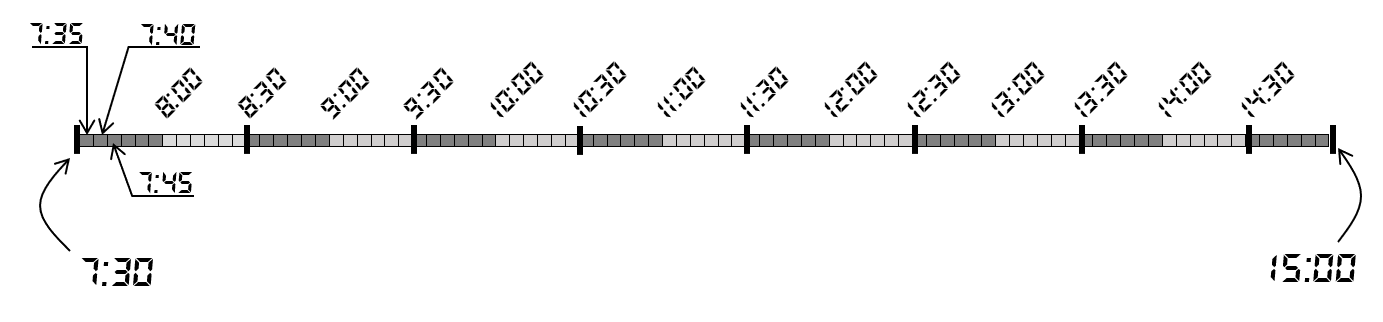
\includegraphics[width=\linewidth]{tiempo-disccreto}
		\caption{Tiempo discreto con \textit{slots} de 5 minutos}
		\label{fig:timepo-disccreto}
	\end{subfigure}

	\caption{Ilustración de la discretización del tiempo}
\end{figure}

Con todo, la representación de una solución es de la forma de la \autoref{fig:3:ejemplo-distribucion-inicial}

\subsection{Fase 1: Inicialización de Soluciones} \label{sec:3:inicializacion-soluciones}

La fase de inicialización toma como entrada la planificación inicial, la planificada para el día y que ya no tiene validez debido a la incidencia; junto a los datos relativos a la incidencia que son:

\begin{itemize}
	\item Hora a la que se produce la incidencia.
	\item Tipo de incidencia.
	\item Si la incidencia es por un cambio imprevisto de sectorización, la nueva sectorización.
	\item Si la incidencia es por una baja de un trabajador, hora de la baja y los datos del trabajador y, opcionalmente, hora del alta y datos del trabajador (puede ser el mismo u otro que no forme parte del turno inicial).
\end{itemize}

\begin{figure}[htbp]
	\centering
	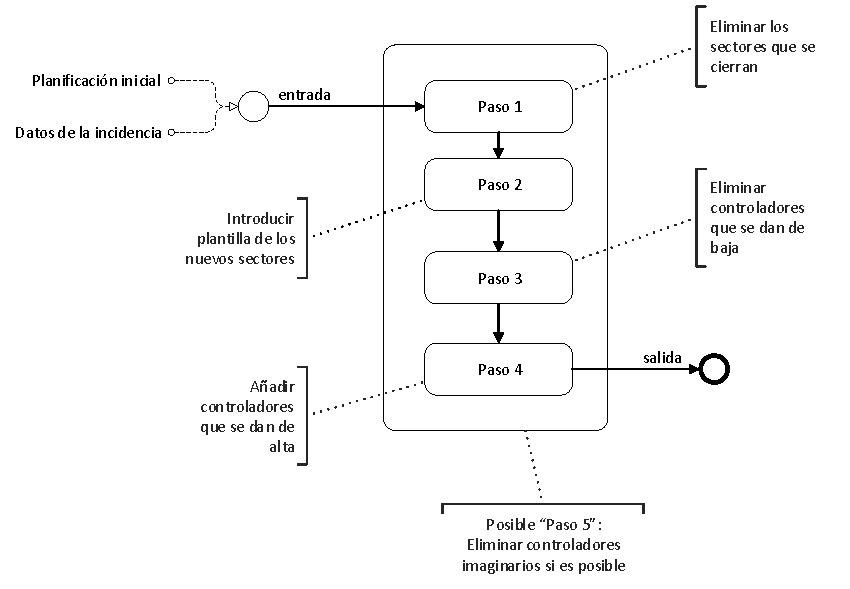
\includegraphics[width=\linewidth]{Esquema-Fase-1-extendido}
	\caption{Diagrama de flujo del funcionamiento de la Fase 1}
	\label{fig:3:esquema-fase-1}
\end{figure}

Con esos datos, la \faseuno{} deberá convertir la planificación inválida en una \textit{solución incial}, que 
emplearemos como punto de partida para el sistema de búsqueda inteligente que es la \fasedos{}. Para ello distinguimos dos tipos de tareas, las relativas a la incidencia por cambio de sector (pasos 1 y 2) y las relativas a las bajas y altas de los trabajadores (pasos 3 y 4). Los pasos pueden verse esquemáticamente en la \autoref{fig:3:esquema-fase-1}.
Adicionalmente, un quinto paso fue planteado para poder facilitar la tarea de la \fasedos{}, que consistía en reducir el numero de controladores añadidos artificialmente en los pasos anteriores moviendo carga de trabajo a otros que la soporten heurísticamente. Finalmente no fue implementada y fue añadida como trabajo futuro.
\\

En la figura \autoref{fig:3:ejemplo-distribucion-inicial} se muestra cómo sería una posible planificación inicial. En éste caso ha sido creada en base a \textit{plantillas} o \textit{estadillos}, que es el método empleado habitualmente por el personal para crear la planificación. Consiste en la repetición de un patrón conformado por tres 
controladores para un sector, en el que se suceden trabajo en puesto planificador, trabajo en puesto ejecutivo y descanso con un desfase en incremento para cada controlador, forma que en cada instante de tiempo (imagínese una línea transversal) habrá un controlador en puesto ejecutivo, otro en planificador y otro descansado. \gls{CRIDA} sabe que el uso de estas plantillas si bien no es lo mas óptimo es lo más cómodo tanto para la creación manual de la planificación como de cara a no incumplir las restricciones de cada trabajador (ver %TODO: referencias!!).
En las representaciones realizadas, se utilizan identificadores de tres letras en lugar del nombre completo del sector para abreviar y mantener el numero de caracteres contante y se han añadido también colores para una mejor visualización.
\textbf{Las letras en mayúscula (AAA-ZZZ) representan un trabajo en puesto de ejecutivo, mientras que las letras minúsculas (aaa-zzz) indican un trabajo en puesto planificador. Los descansos se representan mediante unos (111).}.
Hemos agrupado slots contiguos tanto de trabajo como descanso identicos, de manera que visualmente sea más cómodo de entender. Para que las soluciones aquí presentadas tengan validez final, deberíamos añadir indicadores de las horas de los cambios de puesto, sin embargo para éste documento ésto no es realmente importante por lo que podemos omitirlo.
\\

El tipo de plantilla descrito se le denomina $3\times1$ (3 controladores para 1 sector) pero existen otros tipos como $8\times3$ o $4\times1$, no obstante, la más importante para el sistema es la $3\times1$, que será empleada durante esta Fase.

\subsubsection{Paso 1: Eliminar sectores que se cierran}
El primer paso es el encargado de eliminar los sectores que se cierran. Pongamos por ejemplo que tenemos una 
sectorización 5A que pasa a ser una 6C en un momento dado, tal y como se ilustra en la 
\autoref{fig:3:ejemplo-cambio-sectorizacion}. Como ya hemos dicho previamente, nosotros partimos de una planificación inicial como la representada en la \autoref{fig:3:ejemplo-distribucion-inicial}, que con la nueva sectorización queda totalmente inutilizada, pues podemos ver sectores que ya no se encuentran abiertos a partir del punto de cambio.
\\

\begin{figure}[htbp]
	\centering
	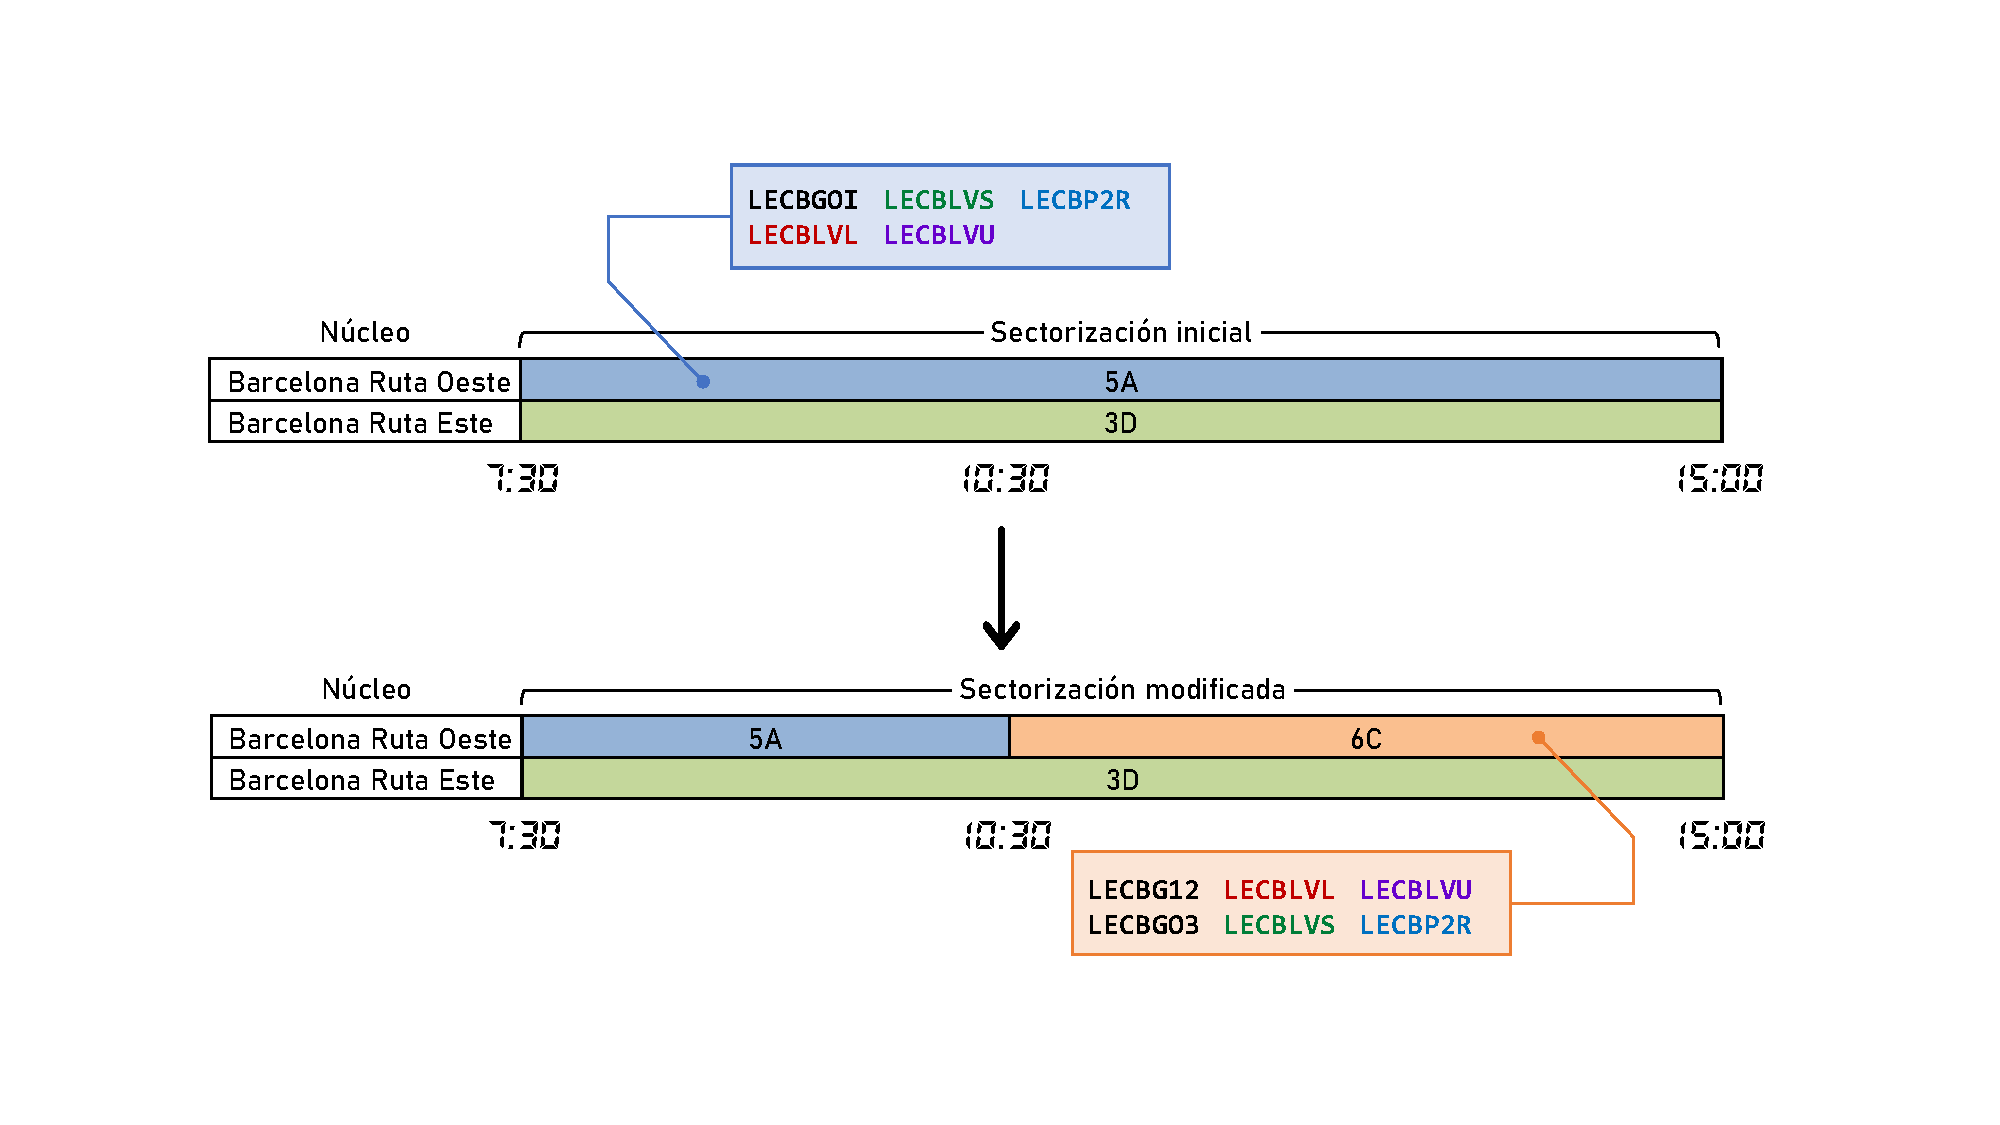
\includegraphics[width=\linewidth]{Ejemplo-cambio-sectorizacion}
	\caption[Ejemplo de cambio de sectorización]{Ejemplo de un posible cambio de sectorización en la Unidad de Control 
	de Barcelona. En color aquellos sectores comunes a ambas sectorizaciones'}
	\label{fig:3:ejemplo-cambio-sectorizacion}
\end{figure}


Identificamos pues, el momento de la incidencia a las 10:30, sin embargo el \textit{momento actual} viene dado a como parte de la entrada. En este caso, han decidido que sea media hora antes de la incidencia, a las 10:00 horas, que equivale al slot numero 30:
\[ 
	10 \,h-7 \,h \,30 \,min = 2 \,h \,30 \,min = \left(2 \, \cancel{h} \times \frac{60 \,min}{1 \,\cancel{h}}\right) 
	\,min + 30\,min = 150 
	\,min 
\]

\[
	150 \,\cancel{min} \times \frac{1\,slot}{5\,\cancel{min}} = 30\,slots
\]
\\

Antes de dicha hora, la planificación no debe ser alterada en ningún caso, pues representa el pasado. En la 
\autoref{fig:3:ejemplo-distribucion-inicial} lo hemos representado con una línea roja. 
\\

En el resto de la planificación, debemos eliminar todos los sectores que no aparecen. Para ello eliminamos aquellos que no pertenezcan a la intersección entre la nueva sectorización y la antigua (es decir, los que siguen en color negro en la \autoref{fig:3:ejemplo-cambio-sectorizacion}). 
Adicionalmente, para obtener una mejor solución inicial y favorecer así a la búsqueda, en el momento de eliminar un sector de la sectorización inicial, tratamos de sustituirlo por uno de los sectores nuevos que se abren (los de la nueva sectorización, los del cuadro naranja en color negro) \textbf{de forma que sean afines de entre sí}, pues el controlador seguirá pudiendo controlarlo sin problemas de acreditación. %FIXME es esto cierto?
\\

Para hacer más eficiente el recorriendo del algoritmo, en lugar de ir slot a slot, podemos agruparlos mientras la sectorización sea la misma. Buscamos un sector afín a cada sector que se cierra y lo sustituimos en todas las apariciones dentro de ése conjunto de slots. Así sucesivamente para cada tramo de slots con la misma sectorización. 
La búsqueda del sector afín es un algoritmo voraz que obtiene el primer sector de entre los que se abren que sea afín al que se cierra, y evitando repeticiones.
\\
\\|
\begin{algorithm}[H]
%	\SetAlgoLined
	\DontPrintSemicolon
	\KwData{
		
		$Sectorizacion_{inicial} = $ conjunto de sectores de la sectorización inicial para cada slot.
			
		$Sectorizacion_{modificada} = $ conjunto de sectores de la sectorización modificada para cada slot.
	}
	\medskip
	
	\ForEach{conjunto de slots con la misma sectorización}{
		$cerrados \leftarrow { Sectorizacion_{modificada}[slot] \setminus Sectorizacion_{inicial}[slot] }$\;
		$abiertos \leftarrow { Sectorizacion_{inicial}[slot] \setminus Sectorizacion_{modificada}[slot] }$\;
		
		\ForEach{$sector_c \in cerrados$}{
			$afin \leftarrow$ buscarPrimerAfin($Sectorizacion_{modificada}[slot]$)\;
			
			\If{$\nexists{afin}$}{
				continue\;	
			} \Else{
				$\forall$ aparición de $sector_c$, sustituir por $afin$\;
			}
		}
			
	}
	
	\caption{Heurística de inicialización: AFINIDADES}
\end{algorithm}


En nuestro ejemplo, solo tenemos un único sector que se cierra, LECBGOI, que sustituiremos, mediante el algoritmo, por el sector LECBG12, que es el primero afín de entre los nuevos abiertos. Mediante esta heurística, evitaremos tener que añadir plantillas (ver \autoref{apartado:3:paso-2}) de todos los sectores nuevos reutilizando los controladores ya existentes.

\subsubsection{Paso 2: Introducir plantillas de los nuevos sectores} \label{apartado:3:paso-2}

Partimos de la lista de sectores nuevos que se abren y que no han sido ya empleados en el paso anterior como sustituto de alguno de los que se cierran. Lo que haremos será añadir una plantilla $3\times1$ como la de la 
\autoref{fig:3:plantilla-3x1} donde alternamos trabajo y descanso a tamaños iguales: el doble de trabajo (uno en cada puesto) por cada uno de descanso. Las plantillas pueden emplearse con cualquier escala de tiempo, por ejemplo 2 horas de trabajo y una de descanso

\begin{figure}
	\centering
	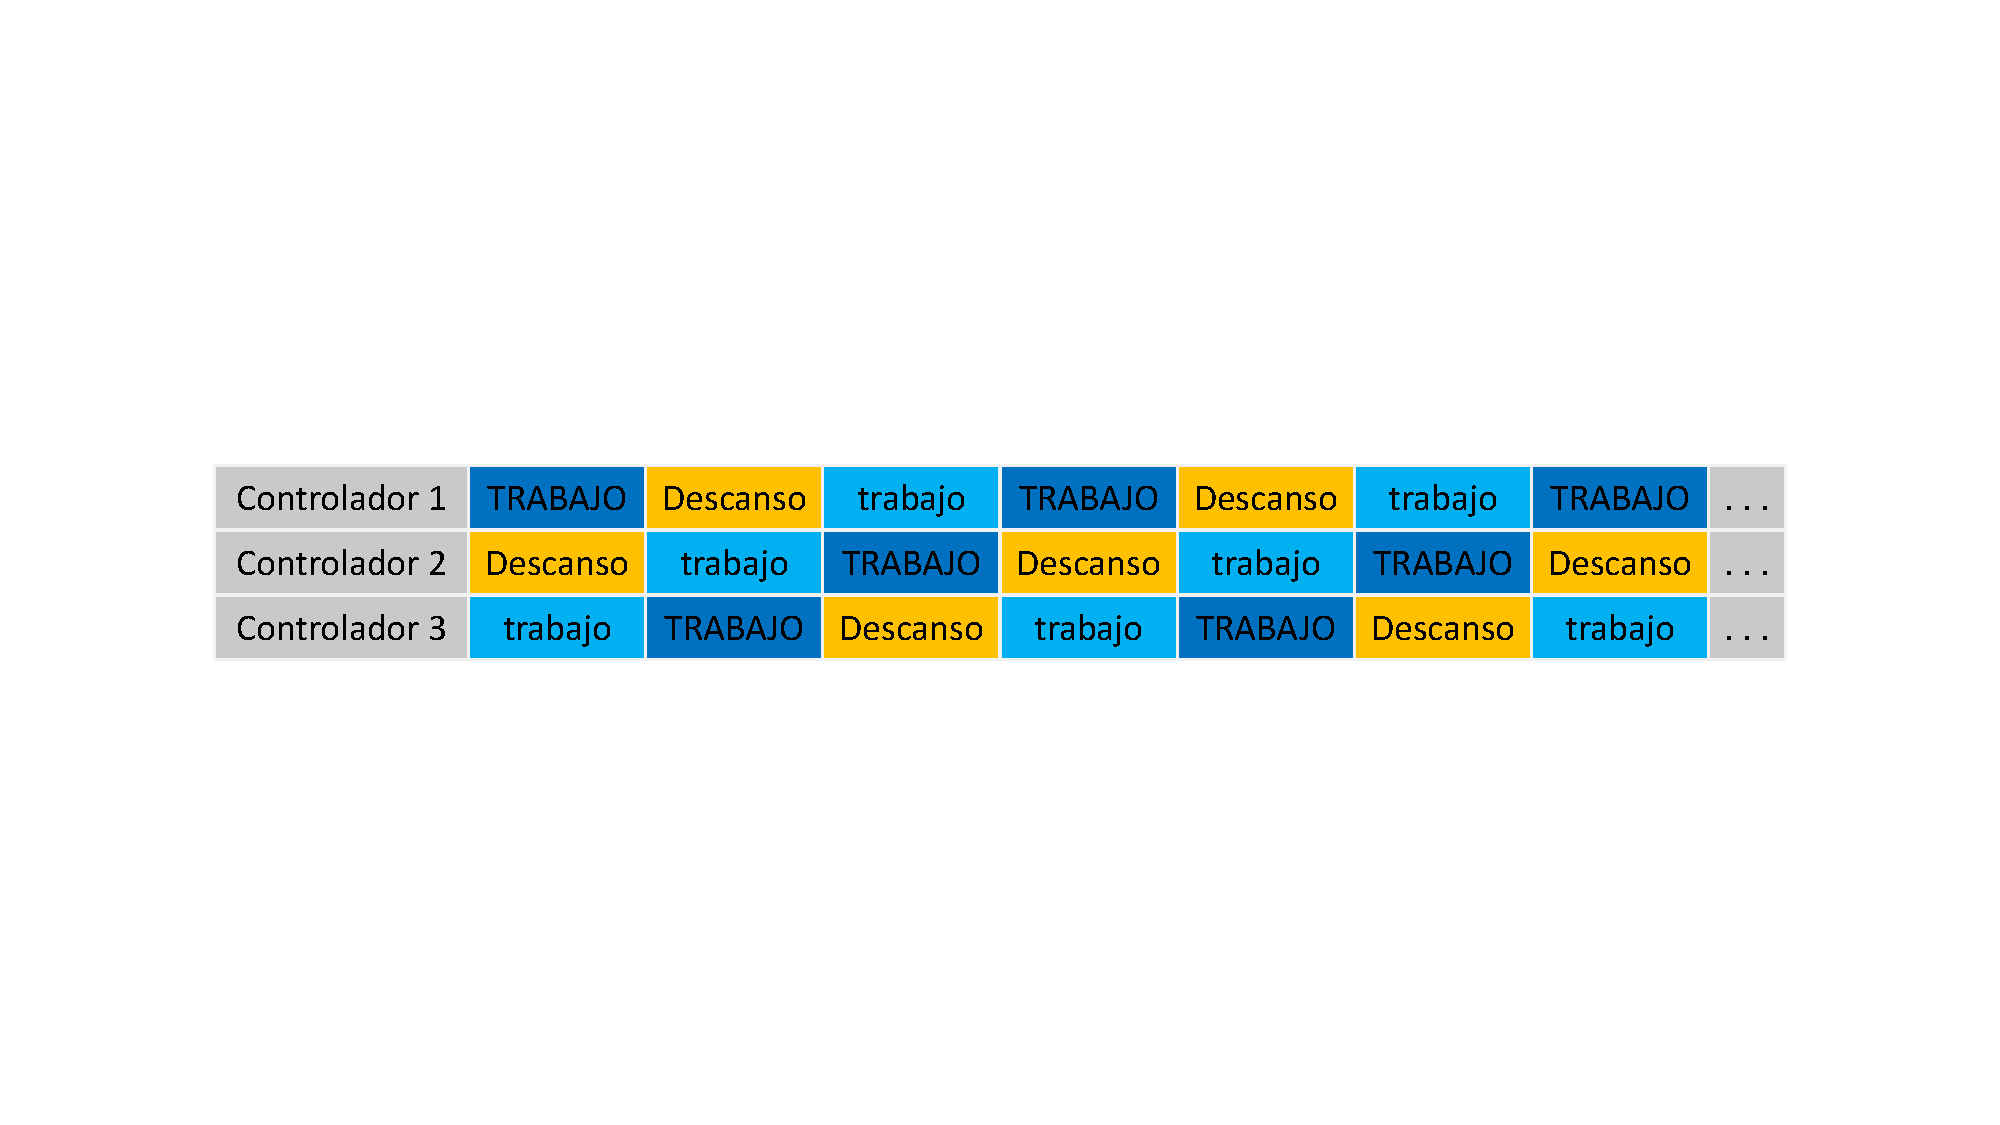
\includegraphics[width=\linewidth]{capitulos/Capitulo3-Metodologia-propuesta/recursos/Plantilla-3x1}
	\caption[Aspecto de una plantilla 3x1]{Aspecto de una plantilla 3x1. Las letras mayúsculas representan trabajo en 
	puesto ejecutivo y las minúsculas en planificador.}
	\label{fig:3:plantilla-3x1}
\end{figure}








